% =====================================================================
% WISA poster paper (Springer LNCS, 12-page limit)
% Build-Configuration-Aware, Triage-Aware Constant-Time Screening for PQC
%
% Compiles on Overleaf as-is (llncs.cls + splncs04.bst are bundled in this
% folder). Locally: pdflatex main && bibtex main && pdflatex main && pdflatex main
%
% TODO(author): fill in the real author name(s) and ORCID before camera-ready.
% TODO(author): verify every reference in references.bib against its source.
% =====================================================================
\documentclass[runningheads]{llncs}

\usepackage[T1]{fontenc}
\usepackage{graphicx}
\usepackage{booktabs}
\usepackage{tabularx}
\usepackage{ragged2e}
\usepackage{amsmath}
\usepackage{amssymb}
\usepackage{xcolor}
\usepackage{tikz}
\usetikzlibrary{arrows.meta,positioning,fit,shapes.geometric}
% hyperref last; remove this line if Overleaf reports a clash with llncs.
\usepackage[hidelinks]{hyperref}
% microtype tightens justification and reduces overfull lines (Springer-safe).
\usepackage{microtype}
% Let long snake_case identifiers (e.g. mlkem768_kyberslash) break after an
% underscore so they do not overflow the margin; no hyphen is inserted.
\renewcommand{\_}{\textunderscore\discretionary{}{}{}}

% Float placement tuning: let more floats share a page and avoid near-empty
% float pages (the 3 tables + figure otherwise pile up at the end).
\setcounter{topnumber}{3}
\setcounter{bottomnumber}{2}
\setcounter{totalnumber}{4}
\renewcommand{\topfraction}{0.92}
\renewcommand{\bottomfraction}{0.5}
\renewcommand{\textfraction}{0.06}
\renewcommand{\floatpagefraction}{0.7}

% Corpus-derived numbers (dudect t/means/n, drop %, cardinalities) are
% single-sourced from docs/corpus/*.csv via scripts/render_paper_tables.py.
% Edit the CSV + re-run the generator; never edit the numbers here by hand.
% tests/test_paper_corpus_sync.py fails if any paper number drifts from the CSV.
% AUTO-GENERATED by scripts/render_paper_tables.py from docs/corpus/*.csv. DO NOT EDIT — edit the CSV + re-run.
\newcommand{\corpusRows}{7}
\newcommand{\corpusFamilies}{3}
\newcommand{\corpusVerdictClasses}{5}
\newcommand{\maxBuildCells}{6}
\newcommand{\dudectLeakyNzero}{13{,}250}
\newcommand{\dudectLeakyNone}{19{,}912}
\newcommand{\dudectLeakyMeanZero}{42.7}
\newcommand{\dudectLeakyMeanOne}{5191.7}
\newcommand{\dudectLeakyT}{181.5}
\newcommand{\dudectLeakyTrunc}{181}
\newcommand{\dudectSafeT}{1.65}
\newcommand{\dropTotalPct}{33.7}
\newcommand{\dropClassZeroPct}{46.6}
\newcommand{\dropClassOnePct}{20.9}
\newcommand{\mlkemDudectT}{5.47}


\begin{document}

\title{Build-Configuration-Aware, Triage-Aware Constant-Time Screening for
Post-Quantum Cryptography}
\titlerunning{Triage-Aware Constant-Time Screening for PQC}

% TODO(author): replace placeholder author / affiliation.
\author{First Author\orcidID{0000-0000-0000-0000}}
\authorrunning{F. Author}
\institute{Hansung University, Seoul, Republic of Korea\\
\email{swhs007@hansung.ac.kr}}

\maketitle

\begin{abstract}
Constant-time (CT) discipline is the standard defense against timing
side channels, but for post-quantum cryptography (PQC) a single
checking technique is not enough. Structural CT checks based on dynamic
taint tracking (Valgrind/Memcheck) detect secret-dependent branches and
memory addresses, yet they pass cleanly over the KyberSlash class of
leaks, where a secret-derived integer division leaks through
variable-latency instructions. Moreover, whether a structural verdict
holds at all can depend on the compiler and optimization level, and
adding more checkers tempts a tool into over-claiming key-recovery
leaks. We present CT-KAT, a fail-closed screening framework that binds
three complementary checkers (Memcheck, a warn-only variable-latency
asm-scan, and the dudect statistical timing test) under one YAML
configuration, indexed by a compiler-by-cflags build matrix, behind a
default-deny triage taxonomy with a cited accepted-variable-time
registry. On a corpus of real PQC and synthetic harnesses, each layer
shows single-coverage of a leak the others miss, and on ML-DSA-65 the
default-deny taxonomy refused to over-claim a leak, instead surfacing
unregistered leak-site functions for human triage. The contribution is
the integration and the triage discipline, not a new attack or a formal
guarantee.

\keywords{post-quantum cryptography \and constant-time \and side-channel
\and KyberSlash \and ML-KEM \and ML-DSA}

\end{abstract}

\section{Introduction}
\label{sec:intro}

NIST has standardized ML-KEM~\cite{fips203} and ML-DSA~\cite{fips204} for
post-quantum cryptography. They are entering widely used libraries and must run in
\emph{constant time}: if secrets influence branches, addresses, or instruction
latency, timing and microarchitectural observations can recover them~\cite{kocher}.
Rejection sampling, modular reduction, and polynomial arithmetic make such
mistakes easy in PQC.

\paragraph{The hook: KyberSlash.}
KyberSlash~\cite{kyberslash} is a family of timing leaks from a secret-dependent
integer division in several Kyber and ML-KEM implementations~\cite{kyber}. Control
flow and access pattern are identical for every input; the leak lives in the
\emph{latency} of one division instruction, which on many platforms depends on its
operands. A classic Valgrind/Memcheck taint screen~\cite{valgrind,ctgrind} flags
secret data reaching a branch or address, but KyberSlash slips past it: the code is
structurally clean while leaking through data-dependent timing.

\paragraph{The problem this creates for tooling.}
KyberSlash exposes three tooling problems. First, single checks have blind spots:
structural taint misses variable-latency instructions, while statistical timing
does not localize the cause. Second, verdicts are build-sensitive: optimization can
remove a debug-only branch or inline a leak into the wrong frame. Third, stacking
alarms tempts over-claiming: many PQC ``failures'' are variable-time by design,
such as ML-DSA rejection sampling~\cite{fips204,dilithium}.

\paragraph{Our approach.}
We present CT-KAT, a fail-closed constant-time screening framework for PQC. Under
one YAML configuration it binds three complementary checkers---a Valgrind/Memcheck
structural taint check, a warn-only assembly scan for variable-latency instruction
candidates, and a dudect-style statistical timing test~\cite{dudect}---and indexes
every structural verdict by a compiler $\times$ cflags build matrix. A failure is
never auto-labeled a key-recovery leak: leak sites are checked against a cited
accepted-variable-time registry, and anything unrecognized remains
\emph{needs-analysis} until a human rules (Figure~\ref{fig:pipeline}).

The phenomena are known: KyberSlash established variable-time division as a leak
class~\cite{kyberslash}, build-sensitivity is folklore, and dudect~\cite{dudect},
ctverif~\cite{ctverif}, and Binsec/Rel~\cite{binsecrel} predate this work. Our
contribution is their \emph{integration}, the \emph{triage discipline} that prevents
over-claiming, and its self-validation on PQClean~\cite{pqclean} targets---most
sharply, the default-deny taxonomy's refusal to over-claim a leak on ML-DSA-65
(Section~\ref{sec:results-coverage}).

\paragraph{Contributions.}
\begin{enumerate}
  \item \textbf{An integrated, build-matrix-indexed framework} binding a structural
    taint check, a variable-latency assembly scan, and a statistical timing test
    across a compiler $\times$ cflags matrix under one YAML config.
  \item \textbf{A default-deny triage taxonomy with a cited registry:} unrecognized
    leak sites stay at needs-analysis, making over-claiming structurally impossible.
  \item \textbf{A validated PQC corpus with the ML-DSA self-validation:} Docker runs
    over three families and five verdict classes (Table~\ref{tab:corpus}), a
    coverage analysis (Table~\ref{tab:coverage}), and a dudect appendix
    (Table~\ref{tab:dudect}).
\end{enumerate}


\section{Background and Related Work}
\label{sec:background}

\subsection{Constant-Time Programming}

A cryptographic implementation is \emph{constant-time} (CT) when execution is
independent of secret data. The usual leak surfaces are secret-dependent
branches, secret-dependent memory addresses, and secret-dependent
variable-latency instructions such as integer division~\cite{kocher}. Defenses
replace these with arithmetic selection, full scans or bit-slicing, and no
secrets in variable-latency instructions. Because compilers can reintroduce or
relocate a leak, CT checking must track the shipped build, not just the source.

\subsection{The Constant-Time Verification Landscape}

\paragraph{Dynamic taint analysis.}
ctgrind~\cite{ctgrind} marks secrets as uninitialized under Valgrind's
Memcheck~\cite{valgrind}, flagging tainted data in a branch or address -- a
precise binary-level check for the first two classes. Its blind spot is
variable-latency arithmetic.

\paragraph{Statistical black-box timing.}
dudect~\cite{dudect} applies a Welch $t$-test to cycle counts for fixed versus
random inputs; a difference signals a leak without modeling why. It is
complementary but noise-sensitive, and it localizes no cause.

\paragraph{Formal and static analysis.}
ct-verif~\cite{ctverif} verifies CT at the LLVM level by reduction to safety,
and Binsec/Rel~\cite{binsecrel} does relational symbolic execution on binaries.
They give stronger guarantees but require more setup and still encode a leak
model. No single technique covers branches, addresses, variable-latency
instructions, and black-box timing at once.

\subsection{Constant-Time Concerns in Post-Quantum Cryptography}

Kyber and Dilithium are lattice schemes~\cite{kyber,dilithium}. NIST standardized
them as ML-KEM and ML-DSA~\cite{fips203,fips204}. Their PQClean
implementations~\cite{pqclean} contain the constructs CT warns about.

KyberSlash~\cite{kyberslash} illustrates this: a division by a public modulus
compiles to a variable-time division on a secret-derived operand. Control flow
and addresses stay constant, so a branch-and-address check reports nothing; the
leak lives in the variable-latency class a Valgrind-style check cannot see.

Yet not every data-dependent timing is a defect. Dilithium signing uses rejection
sampling, so iteration count varies by design; FIPS~204 prescribes this, and the
variation is not a long-term-key leak. Distinguishing accepted behavior from a
genuine leak requires triage, not binary pass/fail.

\subsection{The Gap We Address}

The individual phenomena are known: KyberSlash division, build-sensitive CT, and
dudect timing. Missing is applying complementary checkers under one configuration
and build matrix, then reducing their output through default-deny triage. The
pipeline is Figure~\ref{fig:pipeline}; coverage and verdict classes are
Tables~\ref{tab:coverage} and~\ref{tab:corpus}.


% ---- Fig. 1: pipeline -------------------------------------------------
\begin{figure}[htbp]
\centering
% \resizebox guarantees the diagram never overflows \textwidth (it is wider than
% the LNCS text block at natural size). Remove it if you re-tune the TikZ to fit.
\resizebox{\textwidth}{!}{% CT-KAT pipeline (Fig. 1, label fig:pipeline defined in main file).
% Requires TikZ libraries: arrows.meta, positioning, fit, shapes.geometric.
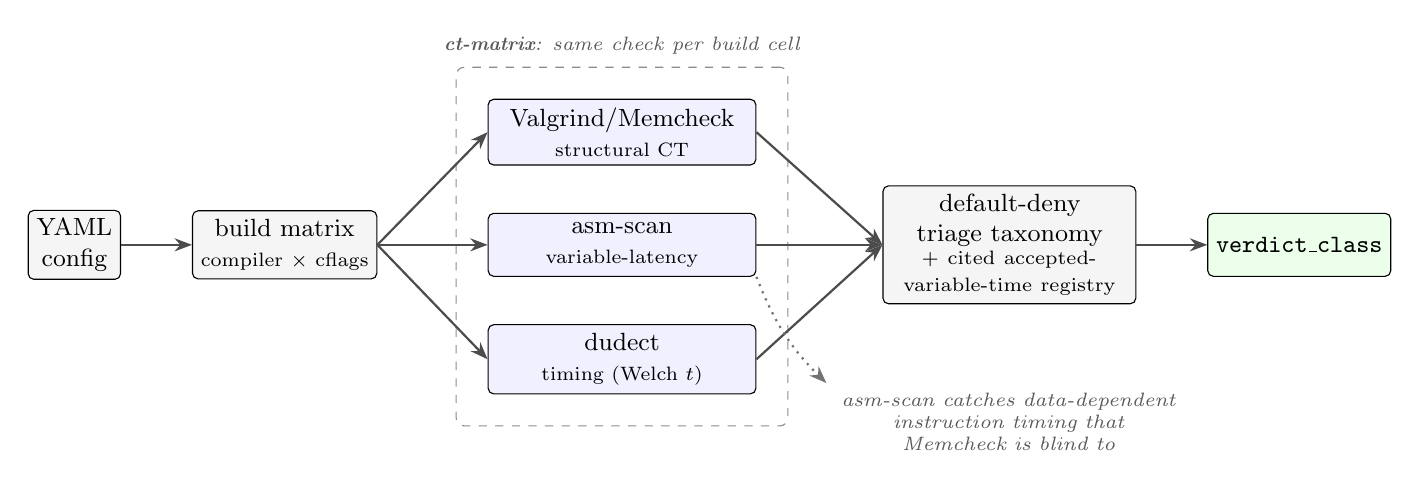
\begin{tikzpicture}[
    font=\small,
    >={Stealth[length=2.2mm]},
    node distance=6mm and 9mm,
    % --- node styles -------------------------------------------------
    stage/.style={
        draw, rounded corners=2pt, align=center,
        minimum height=8mm, inner sep=3pt,
        fill=black!4
    },
    checker/.style={
        draw, rounded corners=2pt, align=center,
        minimum height=8mm, minimum width=34mm, inner sep=3pt,
        fill=blue!6
    },
    verdict/.style={
        draw, rounded corners=2pt, align=center,
        minimum height=8mm, inner sep=3pt,
        fill=green!8
    },
    note/.style={
        font=\scriptsize\itshape, align=center, text=black!65
    },
    flow/.style={->, thick, black!70},
    grp/.style={draw, dashed, rounded corners=3pt, inner sep=4mm, black!45}
]

% --- inputs -------------------------------------------------------
\node[stage] (yaml) {YAML\\config};
\node[stage, right=of yaml] (matrix)
    {build matrix\\\scriptsize compiler $\times$ cflags};

% --- three parallel checkers (stacked vertically) -----------------
\node[checker, right=14mm of matrix] (asm) {asm-scan\\\scriptsize variable-latency};
\node[checker, above=of asm] (mc) {Valgrind/Memcheck\\\scriptsize structural CT};
\node[checker, below=of asm] (dud) {dudect\\\scriptsize timing (Welch $t$)};

% dashed group around the three checkers
\node[grp, fit=(mc)(asm)(dud)] (checkers) {};
\node[note, above=1pt of checkers.north] {\textbf{ct-matrix}: same check per build cell};

% --- triage + registry -------------------------------------------
\node[stage, right=16mm of asm, text width=30mm] (triage)
    {default-deny\\triage taxonomy\\\scriptsize{+ cited accepted-}\\[-1pt]
     \scriptsize{variable-time registry}};

% --- verdict ------------------------------------------------------
\node[verdict, right=of triage] (verdict)
    {\texttt{verdict\_class}};

% --- main flow arrows --------------------------------------------
\draw[flow] (yaml) -- (matrix);
\draw[flow] (matrix.east) -- (mc.west);
\draw[flow] (matrix.east) -- (asm.west);
\draw[flow] (matrix.east) -- (dud.west);

\draw[flow] (mc.east)  -- (triage.west);
\draw[flow] (asm.east) -- (triage.west);
\draw[flow] (dud.east) -- (triage.west);

\draw[flow] (triage) -- (verdict);

% --- asm-scan annotation: catches what Memcheck is blind to -------
\node[note, below=10mm of triage.south,  text width=44mm, anchor=north] (asmnote)
    {asm-scan catches data-dependent\\
     instruction timing that\\
     Memcheck is blind to};
\draw[->, dotted, thick, black!55]
    (asm.south east) to[bend right=12] (asmnote.north west);

\end{tikzpicture}
}
\caption{CT-KAT pipeline: one YAML config drives a compiler$\times$cflags build
matrix feeding three checkers (Valgrind/Memcheck, asm-scan, dudect); results pass
through a default-deny triage taxonomy with a cited accepted-variable-time
registry to a \texttt{verdict\_class}.}
\label{fig:pipeline}
\end{figure}

\section{Framework Design}
\label{sec:design}

CT-KAT (invoked as \texttt{ctkat}) is a fail-closed CT screening framework for
PQC. It binds three complementary checkers under one declarative configuration,
sweeps every harness across a compiler${}\times{}$optimization build matrix, and
routes every finding through a default-deny triage taxonomy backed by a cited
registry of accepted variable-time behavior. The goal is not to prove the
absence of leaks --- no dynamic tool can --- but to make screening honest: each
checker covers a leak class the others miss, the verdict is reported per build,
and a detected CT failure is never silently promoted to a key-recovery leak. The
pipeline (Fig.~\ref{fig:pipeline}) spans configuration (\S\ref{ssec:config}),
checkers (\S\ref{ssec:checkers}), the build sweep (\S\ref{ssec:matrix}), and
triage (\S\ref{ssec:triage}).

\subsection{Unified Configuration and Pipeline}
\label{ssec:config}

One YAML file describes a run: the target harnesses (each a small driver calling
one cryptographic operation, e.g.\ a decapsulation), the secret input regions to
track, the named build configurations, and per-layer options. As the single
source of truth it fixes the build flags, tainted regions, and timing parameters
together, so the measured configuration cannot drift from the assumed one. Each
harness is compiled once per build cell (\S\ref{ssec:matrix}), screened by the
three layers (\S\ref{ssec:checkers}), and reduced by triage
(\S\ref{ssec:triage}) to one \texttt{verdict\_class}.

\subsection{Three Checker Layers}
\label{ssec:checkers}

CT side channels in PQC share no single observable signature, so CT-KAT composes
three checkers, each for a leak class the others cannot see.

\paragraph{Layer 1: structural CT check (Valgrind/Memcheck).}
The classic dynamic-taint approach, after ctgrind~\cite{ctgrind} on
Memcheck~\cite{valgrind}: secret inputs are marked undefined, and Memcheck
reports when a secret-derived value reaches a control-flow branch or a memory
address --- the constructs behind the canonical cache- and branch-timing
leaks~\cite{kocher}. It checks program \emph{structure}, not instruction
\emph{latency}, so a secret-dependent variable-latency division passes it clean.

\paragraph{Layer 2: variable-latency instruction scan (asm-scan).}
\texttt{asm-scan} closes that gap: a warn-only static scan over the emitted
assembly, run across optimization levels, flagging \emph{candidate}
variable-latency instructions --- chiefly integer division and remainder, whose
amd64 latency depends on operands. The KyberSlash class~\cite{kyberslash} is
exactly such a secret-derived division that Memcheck passes clean. It stays
warn-only because the divisor may be public; the public-versus-secret split is
resolved in triage (\S\ref{ssec:triage}).

\paragraph{Layer 3: black-box statistical timing (dudect).}
A black-box test after dudect~\cite{dudect}: it runs the harness on two input
classes and applies a Welch $t$-test to the cycle counts; a large $|t|$ means
the running time depends on the input class, hence the secret. Needing no model
of why a leak occurs, it catches timing dependence with no structural branch and
no recognizable variable-latency instruction. Being measurement-based it is
environment-sensitive: under our virtualized image it can report
environment-induced noise, which it surfaces loudly. The three layers detect
disjoint leak classes --- structural, instruction latency, end-to-end timing ---
so their union is the coverage.

\subsection{Build-Configuration Sweep (ct-matrix)}
\label{ssec:matrix}

A constant-time property belongs to the \emph{compiled} program: the compiler
may remove a secret-dependent branch at one optimization level, or inline a
function so a finding lands in a different frame, making a single-build verdict
unsound. \texttt{ct-matrix} recompiles each harness under every named build
configuration and re-runs the \emph{same} structural check per cell, reporting
the verdict as a function of the build. The matrix is indexed by compiler and
named cflags; our image provides gcc~13.3.0 and clang~18.1.3, giving up to six
cells. The three gcc configurations are \texttt{debug}
(\texttt{-O0 -g -fno-inline -fno-omit-frame-pointer}, disabling inlining so
findings name their precise leak-site function), \texttt{release}
(\texttt{-O2 -g -fno-omit-frame-pointer -fno-lto}), and \texttt{size}
(\texttt{-Os}, otherwise as release). Two phenomena make the sweep load-bearing:
a branch present at \texttt{-O0} can be removed at \texttt{-O2}/\texttt{-Os},
flipping the verdict; and inlining blurs attribution, so \texttt{-O0 -fno-inline}
names the true leak-site function while optimized builds merge it into a parent
frame. CT-KAT unions the leak-site functions and treats the debug build as
authoritative for triage while reporting build-dependence.

\subsection{Default-Deny Triage Taxonomy}
\label{ssec:triage}

Over-claiming every structural failure as a key-recovery leak is dangerous for
PQC, since several schemes are variable-time \emph{by design} --- e.g.\ the
rejection-sampling loops of ML-DSA~\cite{fips204,dilithium}, whose iteration
count depends on a fresh per-signature nonce. CT-KAT assigns each harness exactly
one \texttt{verdict\_class}:
\begin{description}
  \item[\texttt{robust}:] all checkers pass across the matrix.
  \item[\texttt{ct-clean-untriaged}:] structural pass; another layer's candidate
        (e.g.\ a division) is untriaged.
  \item[\texttt{varlat-secret-risk}:] structural pass, but \texttt{asm-scan}
        flags a \emph{secret-derived} variable-latency instruction (the
        KyberSlash case).
  \item[\texttt{build-sensitive-ct}:] the structural verdict is unstable across
        the matrix.
  \item[\texttt{accepted-variable-time}:] structural fail, but \emph{every}
        leak-site function is a registered, cited design behavior.
  \item[\texttt{needs-analysis}:] structural fail with some unregistered
        leak-site function; a human must rule.
  \item[\texttt{ct-leak}:] a confirmed leak, reachable \emph{only} by explicit
        human verdict; never assigned automatically.
\end{description}

The \texttt{accepted-variable-time}/\texttt{needs-analysis} boundary is a cited
registry (\texttt{docs/accepted\_variable\_time.md}): each entry records a
function whose secret-dependent timing is an analyzed-safe design behavior, with
a checkable citation. If \emph{all} leak-site functions are registered the
harness is \texttt{accepted-variable-time}; if \emph{any} is unrecognized it
stays \texttt{needs-analysis} --- never silently accepted, never silently
promoted to a leak. Section~\ref{sec:results-coverage} shows this default-deny
invariant at work on real ML-DSA-65.


\section{Corpus and Methodology}
\label{sec:method}

\subsection{Reproducible environment}

All results are real runs in one pinned container: Ubuntu~24.04 on
\texttt{amd64}, GCC~13.3.0, Clang~18.1.3, Valgrind (Memcheck). A verdict can
depend on compiler and optimization level, so one without the exact compiler
version is under-specified. The suite has 381 passing and 3 skipped tests; skips
need a native (non-emulated) timing environment.

\subsection{Corpus design}

The corpus pairs each layer with a case \emph{only} that layer flags, grounding
every verdict class: real PQClean targets~\cite{pqclean} plus synthetic
controls (Table~\ref{tab:coverage}, per-feature map;
Table~\ref{tab:corpus}, verdict-class corpus).

\paragraph{Real PQC targets.}
For ML-KEM-768 (FIPS~203~\cite{fips203}, \texttt{mlkem768}, harness
\texttt{kem\_dec}) we screen the plain build and a
KyberSlash~\cite{kyberslash} variable-time-division variant
(\texttt{mlkem768\_kyberslash}). The plain build passes structurally
everywhere; \texttt{asm-scan}'s FIPS~202/Keccak division candidates triage
\emph{public} (constant absorb rate). KyberSlash is the key case: Memcheck
passes it clean---no secret-tainted branch or address---yet it leaks through a
secret-derived integer division only \texttt{asm-scan} surfaces.

\paragraph{Synthetic controls.}
Three harnesses isolate one phenomenon each. \texttt{toy\_lookup}'s
\texttt{leaky} variant (\texttt{out[i]=sbox[secret[i]]}) is a cache-timing leak
Memcheck flags across all six builds; \texttt{safe} is robust.
\texttt{ct\_matrix\_flip}'s secret-dependent branch is optimizer-removed: it
fails under GCC debug (\texttt{-O0}) but passes under release (\texttt{-O2}) and
size (\texttt{-Os}). \texttt{toy\_dudect} is a timing control, no structural
branch (Table~\ref{tab:dudect}).

\subsection{How a row is produced}

Each row follows one pipeline (Fig.~\ref{fig:pipeline}) from one YAML config.
\texttt{ct-matrix} recompiles per cell of the compiler~$\times$ named-cflags
matrix (up to six cells, GCC and Clang) using the debug/release/size
configurations of Section~\ref{ssec:matrix}, re-running the \emph{same} check in
each. \texttt{asm-scan} runs warn-only over object code; public
variable-latency candidates are recorded, any unrecognized leak site holds the
row at \texttt{needs-analysis}, and the default-deny taxonomy never auto-promotes
a structural failure to a leak. Optionally \texttt{dudect}~\cite{dudect} (a Welch
$t$-test on cycle counts) runs on timing distributions. The ML-DSA-65 row
(\texttt{mldsa65}, \texttt{sign}) is the central honest result: its structural
check fails, but default-deny holds it at \texttt{needs-analysis} rather than
declaring a leak (Section~\ref{sec:results-coverage}).

\subsection{Merging the evidence}

Structural and \texttt{asm-scan} signals are per build cell, the timing test per
target. A script merges them, collapsing structural results into one verdict per
target (build-sensitive when verdicts vary) and attaching triaged findings:
Table~\ref{tab:corpus}, seven rows, three families, five verdict classes. The timing layer is in the dudect appendix (Table~\ref{tab:dudect}).


% ---- Coverage table: per-feature single-coverage ---------------------
\begin{table}[htbp]
\centering
\caption{Per-feature single-coverage: each layer flags a corpus case the others
miss --- the figure that justifies every layer.}
\label{tab:coverage}
\setlength{\tabcolsep}{4pt}
\renewcommand{\arraystretch}{1.15}
\footnotesize
\begin{tabular}{@{}>{\raggedright\arraybackslash}p{2.0cm} >{\raggedright\arraybackslash}p{2.5cm} >{\raggedright\arraybackslash}p{2.6cm} >{\raggedright\arraybackslash}p{3.2cm}@{}}
\toprule
Tool layer & What only it catches & Single-coverage case & Evidence\\
\midrule
Valgrind taint & secret branch / memory address &
\texttt{toy\_lookup} \texttt{leaky} (S-box read) &
\texttt{ct-leak}: FAIL, all \maxBuildCells{} builds\\
asm-scan & secret division latency (Memcheck-blind) &
KyberSlash ML-KEM &
\texttt{varlat-secret-risk}: ct PASS, asm FAIL\\
ct-matrix & verdict flips per build &
\texttt{ct\_matrix\_flip} \texttt{leaky} &
\texttt{build-sensitive-ct}: \texttt{-O0} FAIL, \texttt{-O2}/\texttt{-Os} PASS\\
dudect & timing leak, no branch &
\texttt{toy\_dudect} \texttt{leaky} &
FAIL $|t|{=}\dudectLeakyT$ vs PASS $\dudectSafeT$\\
default-deny & ct FAIL not yet confirmed &
ML-DSA-65 (\texttt{sign}) &
\texttt{needs-analysis}: refused to over-claim\\
\bottomrule
\end{tabular}
\end{table}

% ---- Ablation/miss support table -------------------------------------
\begin{table}[htbp]
\centering
\caption{Ablation/miss evidence: each omitted layer has a concrete corpus miss.
This supports Table~\ref{tab:coverage} without replacing its single-coverage
claim.}
\label{tab:ablation}
\footnotesize
\setlength{\tabcolsep}{4pt}
\begin{tabular}{@{}>{\raggedright\arraybackslash}p{2.4cm}
                  >{\raggedright\arraybackslash}p{3.8cm}
                  >{\raggedright\arraybackslash}p{4.8cm}@{}}
\toprule
Layer omitted & Demonstrated miss & Evidence\\
\midrule
% AUTO-GENERATED by scripts/render_paper_tables.py from docs/corpus/*.csv. DO NOT EDIT; edit the CSV + re-run.
\texttt{Valgrind taint} & secret-indexed memory leak & \texttt{toy\_lookup/leaky} (\texttt{ct-leak})\tabularnewline
\texttt{asm-scan} & KyberSlash secret-derived division & \texttt{mlkem768\_kyberslash/kem\_dec} (\texttt{varlat-secret-risk})\tabularnewline
\texttt{ct-matrix} & build-dependent verdict flip & \texttt{ct\_matrix\_flip/leaky} (\texttt{build-sensitive-ct})\tabularnewline
\texttt{dudect} & black-box timing leak & \texttt{toy\_dudect/leaky} (FAIL $|t|=181.5$)\tabularnewline
\texttt{default-deny} & ML-DSA over-claim & \texttt{mldsa65/sign} (\texttt{needs-analysis})\tabularnewline
\bottomrule
%
\end{tabular}
\end{table}

% ---- Verdict-class corpus table --------------------------------------
\begin{table}[htbp]
\centering
\caption{Verdict-class corpus: \corpusRows{} harness rows, \corpusFamilies{}
families, \corpusVerdictClasses{} verdict classes, rendered from the committed
corpus CSVs with compiler/version provenance recorded per build cell.}
\label{tab:corpus}
\scriptsize
\setlength{\tabcolsep}{2pt}
\begin{tabular}{@{}>{\raggedright\arraybackslash}p{1.25cm}
                  >{\raggedright\arraybackslash}p{2.55cm}
                  >{\raggedright\arraybackslash}p{1.1cm}
                  >{\centering\arraybackslash}p{1.45cm}
                  >{\raggedright\arraybackslash}p{1.35cm}
                  >{\raggedright\arraybackslash}p{2.75cm}@{}}
\toprule
Family & Target & Harness & ct (matrix) & varlat & \texttt{verdict\_class}\\
\midrule
% rows generated from docs/corpus/corpus_summary.csv — see preamble note.
% AUTO-GENERATED by scripts/render_paper_tables.py from docs/corpus/*.csv. DO NOT EDIT — edit the CSV + re-run.
ML-KEM & \texttt{mlkem768} & \texttt{kem\_dec} & PASS & public & \texttt{robust}\\
ML-KEM & \texttt{mlkem768\_kyberslash} & \texttt{kem\_dec} & PASS & secret-risk & \texttt{varlat-secret-risk}\\
ML-DSA & \texttt{mldsa65} & \texttt{sign} & FAIL & public & \texttt{needs-analysis}\\
synthetic & \texttt{toy\_lookup} & \texttt{leaky} & FAIL & none & \texttt{ct-leak}\\
synthetic & \texttt{toy\_lookup} & \texttt{safe} & PASS & none & \texttt{robust}\\
synthetic & \texttt{ct\_matrix\_flip} & \texttt{leaky} & FAIL/PASS & none & \texttt{build-sensitive-ct}\\
synthetic & \texttt{ct\_matrix\_flip} & \texttt{safe} & PASS & none & \texttt{robust}\\
%
\end{tabular}
\end{table}

% ---- ML-DSA attribution support table --------------------------------
\begin{table}[htbp]
\centering
\caption{ML-DSA-65 attribution split: debug cells show only registered
accepted-variable-time functions; optimized cells surface the unregistered names
that keep the row at \texttt{needs-analysis}.}
\label{tab:mldsa}
\footnotesize
\setlength{\tabcolsep}{4pt}
\begin{tabular}{@{}>{\raggedright\arraybackslash}p{2.2cm}
                  >{\raggedright\arraybackslash}p{5.4cm}
                  >{\raggedright\arraybackslash}p{3.5cm}@{}}
\toprule
Build cells & Functions surfaced & Triage meaning\\
\midrule
% AUTO-GENERATED by scripts/render_paper_tables.py from docs/corpus/*.csv. DO NOT EDIT; edit the CSV + re-run.
\texttt{-O0 -fno-inline} & \texttt{make\_hint}; \texttt{poly\_challenge}; \texttt{poly\_chknorm} & registered rejection-sampling behavior\tabularnewline
\texttt{-O2/-Os} & adds \texttt{crypto\_sign\_signature\_ctx}; \texttt{pack\_sig} & held at \texttt{needs-analysis}\tabularnewline
\bottomrule
%
\end{tabular}
\end{table}

% ---- dudect appendix table -------------------------------------------
\begin{table}[htbp]
\centering
\caption{dudect timing appendix on \texttt{toy\_dudect} (cycle counts, Welch
$t$). Beside the corpus rather than in it, since dudect is timing-keyed, not
ct-matrix-keyed.}
\label{tab:dudect}
\footnotesize
\begin{tabular}{@{}llrrrrrl@{}}
\toprule
Target & Harness & $n_0$ & $n_1$ & mean$_0$ & mean$_1$ & $|t|$ & status\\
\midrule
% rows generated from docs/corpus/dudect_appendix.csv — see preamble note.
% AUTO-GENERATED by scripts/render_paper_tables.py from docs/corpus/*.csv. DO NOT EDIT — edit the CSV + re-run.
\texttt{toy\_dudect} & \texttt{leaky} & 13250 & 19912 & 42.7 & 5191.7 & 181.5 & FAIL\\
\texttt{toy\_dudect} & \texttt{safe} & 19578 & 19773 & 10269.3 & 10267.9 & 1.65 & PASS\\
%
\end{tabular}
\end{table}

\section{Results}
\label{sec:results}

We evaluate CT-KAT on seven harness rows across ML-KEM, ML-DSA, and synthetic
controls, under up to six gcc/clang build cells. The committed corpus CSVs record
build-cell provenance. Table~\ref{tab:coverage} shows each layer catches a case
the others miss; Table~\ref{tab:corpus} grounds verdict classes; Table~\ref{tab:dudect}
is the timing appendix. Tables~\ref{tab:ablation} and~\ref{tab:mldsa} add the
two supporting checks: what each omitted layer misses, and why ML-DSA remains
\texttt{needs-analysis}.

\subsection{Per-feature single-coverage}
\label{sec:results-coverage}

Table~\ref{tab:coverage} names, per layer, one case that \emph{only} it flags.
Two are the paper's spine.

\paragraph{(i) asm-scan: structural CT alone is insufficient.}
The KyberSlash harness passes Memcheck clean: no secret-tainted branch or
address. Yet asm-scan flags a
secret-derived integer division---the KyberSlash class~\cite{kyberslash}---whose
latency is data-dependent. Triage marks it secret-derived, giving
the risk verdict in Table~\ref{tab:corpus}; a Memcheck-only deployment would
ship it as clean.

\paragraph{(ii) Default-deny triage: a structural FAIL the tool refused to
call a leak.}
On real ML-DSA-65 (\texttt{mldsa65} / \texttt{sign}) structural checking fails.
Three --- \texttt{poly\_chknorm}, \texttt{make\_hint}, and
\texttt{poly\_challenge} --- are registered rejection-sampling behavior required
by ML-DSA~\cite{fips204,dilithium}. Two are not:
\texttt{crypto\_sign\_signature\_ctx} (optimized-build inlining) and
\texttt{pack\_sig} (a public-signature packer). Default-deny therefore holds the
row at \texttt{needs-analysis}: neither auto-accepting nor over-claiming. The
\texttt{-O0 -fno-inline} cells show only registered functions; optimized cells
surface the two unregistered names (Table~\ref{tab:mldsa}).

\paragraph{The remaining three layers.}
The synthetic controls justify the remaining layers. \texttt{toy\_lookup/leaky}
is a secret-indexed lookup Memcheck flags in all six cells. \texttt{ct\_matrix\_flip/leaky}
fails at \texttt{-O0} but passes at \texttt{-O2}/\texttt{-Os}, exposing
build-sensitive CT. \texttt{toy\_dudect} isolates a timing leak with no structural
branch. No four layers subsume the fifth; Table~\ref{tab:ablation} states the
corresponding miss if each layer is removed.

\subsection{Verdict-class corpus}
\label{sec:results-corpus}

Table~\ref{tab:corpus} grounds every verdict class in a concrete target. Stock
\texttt{mlkem768/kem\_dec}~\cite{pqclean,fips203,kyber} is \texttt{robust}; its
Keccak division candidates triage public. The KyberSlash variant is
\texttt{varlat-secret-risk}; ML-DSA contributes \texttt{needs-analysis}; and
synthetic controls cover \texttt{ct-leak} and \texttt{build-sensitive-ct}. The
tool never auto-declares \texttt{ct-leak}: an explicit human verdict is required.
Together the tables make the framework layer-justified in this corpus and
validated on concrete runs, without claiming formal completeness or leak absence.

\subsection{Statistical timing appendix and its honesty caveat}
\label{sec:results-dudect}

dudect is keyed per target, not per build cell, so it lives beside
Table~\ref{tab:corpus}. The \texttt{toy\_dudect}
rows are unambiguous: \texttt{leaky} ($n_0=\dudectLeakyNzero$,
$n_1=\dudectLeakyNone$, mean cycles $\dudectLeakyMeanZero$ versus
$\dudectLeakyMeanOne$) gives $|t|=\dudectLeakyT$ and a FAIL; \texttt{safe}
gives $|t|=\dudectSafeT$ and a PASS.

We report the caveat because the tool does: the \texttt{leaky} run dropped
$\dropTotalPct\%$ zero-cycle samples, asymmetrically
($\dropClassZeroPct\%$ of class 0 versus $\dropClassOnePct\%$ of class 1), from
QEMU/Docker TSC skew. The large separation ($|t|=\dudectLeakyTrunc$) makes the
FAIL unambiguous, but publication-grade timing should be confirmed natively. The
same warning appears on stock \texttt{mlkem768} ($t=\mlkemDudectT$), read as QEMU
noise rather than a real leak.


\section{Discussion}
\label{sec:discussion}

\paragraph{ML-DSA as a triage stress test.}
The ML-DSA-65 result (Section~\ref{sec:results-coverage}) is a stress test for
conservative triage, not a leak claim. The debug build names only registered
rejection-sampling functions, but optimized builds inline those functions into
\texttt{crypto\_sign\_signature\_ctx} and also surface \texttt{pack\_sig}. CT-KAT
therefore leaves the row at \emph{needs-analysis}: the registry explains part of
the finding, while the build matrix exposes attribution that is too coarse for
automatic acceptance. This is the intended behavior for a screening artifact: it
turns ambiguous evidence into a precise review item rather than a stronger claim.

\paragraph{Why complementary candidate sources, not one.}
KyberSlash shows that structural CT checking and instruction-latency scanning
are genuinely orthogonal: Memcheck~\cite{valgrind,ctgrind} passes the variant
clean while asm-scan surfaces the secret-derived division candidate~\cite{kyberslash}.
Neither refines the other; each sees inputs the other is blind to. A single
checker, however sound on its own class~\cite{ctverif,binsecrel}, would miss the
rest --- which is why the workflow binds several candidate sources before triage.

\paragraph{Limitations.}
The structural and timing checks are dynamic and see only exercised paths;
untaken-branch leaks are out of scope. For KEMs specifically, the structural
harness decapsulates a \emph{valid} ciphertext, so Valgrind covers the normal
path only; the implicit-rejection (Fujisaki--Okamoto) path---an important ML-KEM
leak surface---is not structurally exercised in this corpus and can only be explored
by dudect's \texttt{leak\_target:~fo} timing mode rather than by the structural
check. The dudect test~\cite{dudect} runs
under QEMU/Docker with a noisy cycle counter (Table~\ref{tab:dudect}); large
separations are unambiguous but precise statistics should be confirmed
natively (\texttt{taskset}, frequency scaling off). Asm-scan is candidate-level
and warn-only: flagging a variable-latency instruction~\cite{kocher} is not
proof its operand is secret, so findings feed triage, not a verdict. The
synthetic harnesses isolate one feature each and are deliberately not PQC, and
the corpus covers one ML-KEM~\cite{fips203,kyber} and one
ML-DSA~\cite{pqclean} family. CT-KAT reflects these scope boundaries in its
reports: clean rows are screening results, not absence proofs, and \emph{ct-leak}
requires an explicit human verdict.


\section{Conclusion}
\label{sec:conclusion}

CT-KAT binds three checkers --- a Valgrind/Memcheck structural CT
check~\cite{valgrind,ctgrind}, a warn-only variable-latency asm-scan, and the
dudect statistical timing test~\cite{dudect} --- under one YAML config and
compiler-by-cflags matrix, behind a default-deny triage taxonomy with a cited
accepted-variable-time registry. On the corpus it is
\emph{layer-justified} (each layer single-covers a leak the others miss,
Table~\ref{tab:coverage}), \emph{validated} (verdict classes map to concrete
targets, Tables~\ref{tab:corpus} and~\ref{tab:dudect}), and \emph{honest by
construction}: on ML-DSA-65~\cite{fips204} the taxonomy refused to auto-label a
structural failure as key-recovery, holding the unregistered leak sites at
\emph{needs-analysis} rather than over-claiming. The KyberSlash
case~\cite{kyberslash} shows structural checking alone is insufficient for PQC,
justifying the multi-layer design.

We claim no new attack, guarantee, or absence proof; the phenomena are known,
and the contribution is their integration and triage. Future work broadens the
corpus to Falcon and SPHINCS+ and resolves ML-DSA attribution via a dedicated
\texttt{-fno-inline} build.


\bibliographystyle{splncs04}
\bibliography{references}

\end{document}
